% include the figures path relative to the master file
\graphicspath{ {./content/results/figures/} }
\definecolor{acm}{rgb}{0.8 0.7254901960784313 0.4549019607843137}
\newcommand{\acmColor}{yellow}

\definecolor{ml}{rgb}
{0.3333333333333333  0.6588235294117647 0.40784313725490196}
\newcommand{\mlColor}{green}

\definecolor{other}{rgb}
{0.5058823529411764  0.4470588235294118 0.6980392156862745}
\newcommand{\otherColor}{purple}

\definecolor{db}{rgb}
{0.7686274509803922  0.3058823529411765 0.3215686274509804}
\newcommand{\dbColor}{red}

\definecolor{aov}{rgb}
{0.2980392156862745  0.4470588235294118 0.6901960784313725}
\newcommand{\aovColor}{blue}

\tikzstyle{acmStyle} = [fill=acm]
\tikzstyle{mlStyle} = [fill=ml]
\tikzstyle{otherStyle} = [fill=other]
\tikzstyle{nodeBase} = [ rectangle,rounded corners=2pt]




\begin{figure}[t]
  \centering
  
  \begin{tikzpicture}
  \tikzstyle{noMargin} = [inner sep=0mm, outer sep=0mm]
  \node[noMargin](a){
    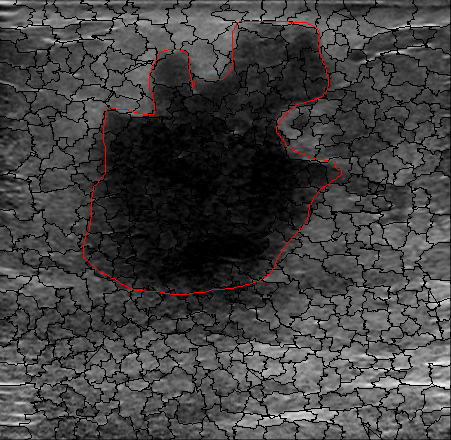
\includegraphics[trim= 20 0 30 0, clip, height=3cm]{goodQSorigin}
  };
  \node[noMargin, right= 3pt of a](b){
    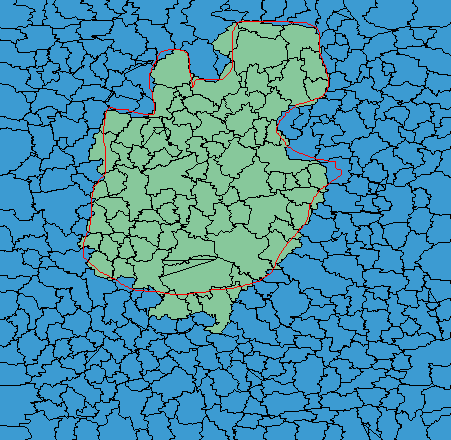
\includegraphics[trim= 20 0 30 0, clip, height=3cm]{goodQSseg}
    };
  \node[noMargin, right= 3pt of b](c){
    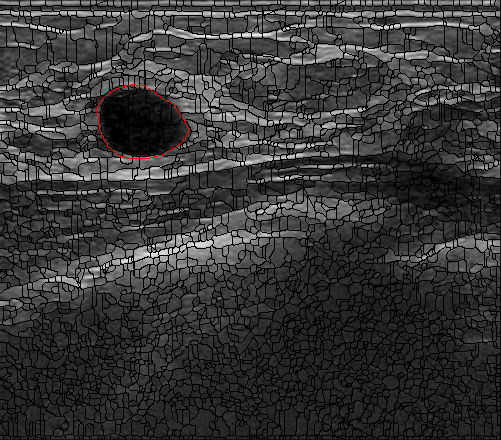
\includegraphics[trim = 0 90 0 0, clip, height=3cm]{fporigin}
  };
  \node[noMargin, right= 3pt of c]{
    \begin{tikzpicture}
      \node[noMargin](d){
      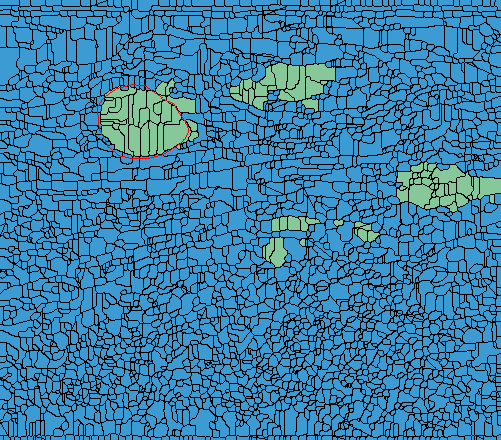
\includegraphics[trim = 0 90 0 0, clip, height=1.2cm]{fpnohom}
      };
      \node[noMargin, below= 5pt of d]{
      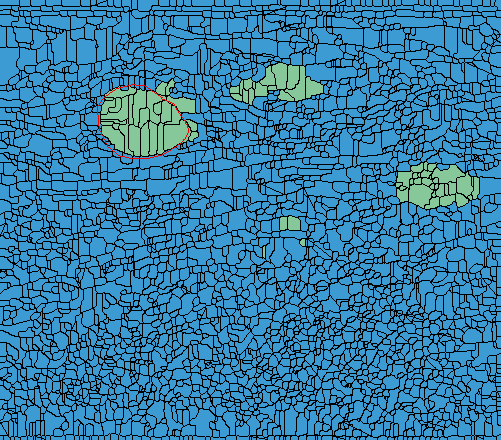
\includegraphics[trim = 0 90 0 0, clip, height=1.2cm]{fpHom}
      };
    \end{tikzpicture}
  };

  \end{tikzpicture}

  \caption{\footnotesize Qualitative results. 
    (a) Example 1: orignal image, super-pixels' delineations and \ac{gt}. 
    (b) Differences between \ac{gt} and the delination resulting from super-pixels' boundary.
    (c) Ex. 2.
    (d) weak $V(\cdot,\cdot)$
    (e) strong $V(\cdot,\cdot)$
    \vspace{-10pt}
    }
  \label{fig:results}
\end{figure}


\section{Method evaluation and comparison} 

\begin{figure}[t]
  \begin{subfigure}[b]{\textwidth}
    {\tiny 
\newcommand{\myCoord}[1]{
  \tikz[remember picture]{\coordinate[remember picture] (#1) at (0,0);
    %\fill[red] (#1) circle[radius=1pt];
  }
}

\newcommand{\drawBox}[5] {
  % draw a colored bar [0..MaxValue] 
  % parameters:
  %  #1 - bar color
  %  #2 - bar width
  %  #3 - bar height
  %  #4 - MaxValue
  %  #5 - actual Value
  \begin{tikzpicture}[baseline=(value.center)]
    \def\w{#2}                   % width of a box
    \def\h{#3}                   % height of a box
    \pgfmathsetmacro{\v}{#5/#4}  % value to display in ratio [0-1]  
    \pgfmathsetmacro{\V}{100*\v} % value to display in percentage   
    \def\x{\v*\w}                % position of the desired value

    % draw rectangle (value dims between color and: white-body, gray-border)
    \draw[draw=#1!\V!gray!] (0,0) rectangle (\w,\h);
    \filldraw[fill=#1!\V!white!, draw=#1!\V!gray!] (0,0) rectangle (\x,\h);
    % display the value
    \path (0,0) -- (0,\h) node[midway,anchor=west] (value) {#5};

%    \draw [blue] (current bounding box.south west) rectangle (current bounding box.north east);
  \end{tikzpicture}
}

\centering
\begin{tabular}{lcccccccccccccccc}
  Method Id\textsuperscript{[ref]}:
              &a\cite{Liu:2010p14328}
              &b\cite{Gao:2012p14336}
              &c\cite{AlemanFlores:2007p14310}
              &d\cite{Huang:2012p14313}
              &e\cite{Madabhushi:2003p6036}
              &f\cite{hao2012combining}
              &g\cite{Zhang:2010p14317}
              &h\cite{Xiao:2002p5639}
              &i\cite{massich2010lesion}
              &j\cite{Shan:2012p14347}
              &k\cite{Yeh:2009p11985}
              &l\cite{Horsch:2001p6028}
              &m\cite{Gomez:2010p14339}
              &n\cite{Huang:2005p11636}
              &o\cite{Huang:2007p6100}
              &p\cite{Cui:2009p14325}\\
  \\\hline \\
  Dataset size:     & 76   & 20   & 32   & 20   & 42   & 480  & 347    & 352  & 25
                    & 120  & 6    & 400  & 50   & 20   & 118  & 488 \\

  techonlogy used for:  &\\
  \quad detection       & \myCoord{Adetect} & \myCoord{Bdetect} & \myCoord{Cdetect} & \myCoord{Ddetect} & \myCoord{Edetect} 
                        & \myCoord{Fdetect} & \myCoord{Gdetect} & \myCoord{Hdetect} & \myCoord{Idetect} & \myCoord{Jdetect}
                        & \myCoord{Kdetect} & \myCoord{Ldetect} & \myCoord{Mdetect} & \myCoord{Ndetect} & \myCoord{Odetect}
                        & \myCoord{Pdetect}\\

  \quad segmetnation    & \myCoord{Aseg} & \myCoord{Bseg} & \myCoord{Cseg} & \myCoord{Dseg} & \myCoord{Eseg} 
                        & \myCoord{Fseg} & \myCoord{Gseg} & \myCoord{Hseg} & \myCoord{Iseg} & \myCoord{Jseg}
                        & \myCoord{Kseg} & \myCoord{Lseg} & \myCoord{Mseg} & \myCoord{Nseg} & \myCoord{Oseg}
                        & \myCoord{Pseg}\\

  \quad post-processing & \myCoord{App} & \myCoord{Bpp} & \myCoord{Cpp} & \myCoord{Dpp} & \myCoord{Epp} 
                        & \myCoord{Fpp} & \myCoord{Gpp} & \myCoord{Hpp} & \myCoord{Ipp} & \myCoord{Jpp}
                        & \myCoord{Kpp} & \myCoord{Lpp} & \myCoord{Mpp} & \myCoord{Npp} & \myCoord{Opp}
                        & \myCoord{Ppp}\\
  \\\hline \\
  \ac{aov} (in \%): & 88.1 & 86.3 & 88.3 & 85.2 & 62.0 & 75.0 & 84.0   & 54.9 & 64.0
                    & 83.1 & 73.3 & 73.0 & 85.0 & 78.6 & 77.6 & 74.5\\
\end{tabular}


\begin{tikzpicture}[remember picture, overlay]
  % single step ACM
  \foreach \x in {Cseg, Cpp, Dpp, Epp, Npp, Opp, Ppp}
  \node[nodeBase, acmStyle, anchor=center] at (\x) {};

  % single step ML
  \foreach \x in {Edetect, Gdetect, Idetect, Pseg}
  \node[nodeBase, mlStyle, anchor=center] at (\x) {};

  % single step Other
  \foreach \x in {Eseg, Iseg, Ipp, Jpp, Kseg, Lseg, Mseg, Mpp, Nseg}
  \node[nodeBase, otherStyle, anchor=center] at (\x) {};

  \node[nodeBase, acmStyle, fit= (Adetect) (Aseg) (App)] {};
  \node[nodeBase, acmStyle, fit= (Bseg)(Bpp)] {};
  \node[nodeBase, mlStyle, fit= (Ddetect)(Dseg)] {};
  \node[nodeBase, mlStyle, fit= (Fdetect)(Fseg)] {};
  \node[nodeBase, mlStyle, fit= (Gseg)(Gpp)] {};
  \node[nodeBase, mlStyle, fit= (Hseg)(Hpp)] {};
  \node[nodeBase, mlStyle, fit= (Jdetect)(Jseg)] {};
  \node[nodeBase, otherStyle, fit= (Odetect)(Oseg)] {};
\end{tikzpicture}
}
    %\caption{\ac{bus} images lesion segmentation strategies compiled from the bulk of the literature: reported quantitative results and methodology highlights.}
    \label{fig:surveyResults:survey}
  \end{subfigure}
  \begin{subfigure}[b]{\textwidth}
    {\tiny \begin{tikzpicture}[scale=.85]


  \def\labels{ c, b, a, p, o, n, m, l, k, j, i, h, g, f, e, d}
  
  \def\reward{88.3,86.3,88.1,74.5,77.6,78.6,85.0,73.0,73.3,83.1,64.0,54.9,84.0,75.0,62.0,85.2}
  \def\dbSize{32,20,76,488,118,20,50,400,6,120,25,352,347,480,42,20}
  \def\dbClass{1,1,2,3,2,1,2,3,1,2,1,3,3,3,1,1}		
  \def\cZoom{3} 
  \def\percentageLabelAngle{90}
  \def\nbeams{16}
  \pgfmathsetmacro\beamAngle{(360/\nbeams)}
  \pgfmathsetmacro\halfAngle{(180/\nbeams)}
  % \def\globalRotation{10}
  \pgfmathsetmacro\globalRotation{\halfAngle}

  % draw manual AOV results
  \filldraw[aov!15!white,even odd rule] (0,0) circle [radius={\cZoom*.852}] (0,0) circle [radius={\cZoom*.8}];
  \draw[thin,color=aov!50!white,dashed] (0,0) circle [radius={\cZoom*.852}] (0,0) circle [radius={\cZoom*.8}];

  % \foreach \x in {.125,.25, ...,1} { \draw[thin]  (0,0) circle [radius={2*\x}]; }
  % draw the radiants with the reference label
  \foreach \n  [count=\ni] in \labels
  {
    \pgfmathsetmacro\cAngle{{(\ni*(360/\nbeams))+\globalRotation}}
    \draw [thin] (0,0) -- (\cAngle:{\cZoom*1}) ;
    \draw	(\cAngle:{\cZoom*1.1})  node[fill=white, inner sep=0pt] {{\tiny \textbf  \n}}; %referencies
  }

  % draw the % rings 
  \foreach \x in {12.5,25, ...,100} 
  \draw [thin,color=gray!50] (0,0) circle [radius={\cZoom*\x/100}];

  \foreach \x in {50,75,100}
  { 
    \draw [thin,color=black!50] (0,0) circle [radius={\cZoom/100*\x}];
    \foreach \a in {0, 180} \draw ({\percentageLabelAngle+\a}:{\cZoom*0.01*\x}) node  [inner sep=0pt,outer sep=0pt,fill=white,font=\fontsize{5}{5}\selectfont]{$\x$};
  }
  
  %% draw our results ring
  \draw [thick,color=black] (0,0) circle [radius={\cZoom*.63}];
  \foreach \a in {0, 180} \draw ({\percentageLabelAngle+\a}:{\cZoom*0.63}) node  [inner sep=0pt,outer sep=0pt,fill=white,font=\fontsize{5}{5}\selectfont]{$62.3$};


  % draw the path of the percentages
  \def\aux{{\reward}}
  \pgfmathsetmacro\origin{\aux[\nbeams-1]} 
  \draw [aov, thick] (\globalRotation:{\cZoom*\origin/100}) \foreach \n  [count=\ni] in \reward { -- ({(\ni*(360/\nbeams))+\globalRotation}:{\cZoom*\n/100}) } ;

  % label all the percentags
  \foreach \n [count=\ni] in \dbSize 
  {
    \pgfmathsetmacro\cAngle{{(\ni*(360/\nbeams))+\globalRotation}}
    \pgfmathsetmacro\nreward{\aux[\ni-1]}
%    \draw (\cAngle:{\cZoom*1.4}) node[align=center] {{\color{aov}\nreward $\%$} \\ {\color{db}\n} };
  } ;

  % draw the database rose
  \def\dbScale{\09}
  \foreach \n [count=\ni] in \dbClass
  \filldraw[fill=db!20!white, draw=db!50!black]
  (0,0) -- ({\ni*(360/\nbeams)-\halfAngle+\globalRotation}:{\cZoom*\n/9}) arc ({\ni*(360/\nbeams)-\halfAngle+\globalRotation}:{\ni*(360/\nbeams)+\halfAngle+\globalRotation}:{\cZoom*\n/9}) -- cycle;
  \foreach \x in {1,2,3}
  \draw [thin,color=db!50!black,dashed] (0,0) circle [radius={\cZoom*\x/9}];

  %% draw the legend
  \node [anchor=north west,yshift=-6pt] at (-45:\cZoom*1.1){
    \begin{tikzpicture}[font=\tiny]
      \begin{customlegend}[ 
        legend style={ draw=none},
        legend entries={AOV, Our results}
        ]
        \addlegendimage{db,draw=aov,thick,sharp plot}
        \addlegendimage{db,draw=black,thick,sharp plot}
      \end{customlegend}
    \end{tikzpicture}};

  \node [anchor=north east, xshift=-5pt] at (-130:\cZoom*1.1){
    \begin{tikzpicture}[font=\tiny]
      \begin{customlegend}[ 
        legend style={ draw=none},
        legend entries={Dataset, Experts\cite{gerard2013}}
        ]
        \addlegendimage{db,fill=db!20!white, draw=db!60!gray, ybar, ybar legend}
        \addlegendimage{db,fill=aov!15!white,draw=aov,dashed,area legend}
      \end{customlegend}
    \end{tikzpicture}};

  %% draw the domain of each class 
  %\def\puta{	3/0/{\tikz{\node[nodeBase,acmStyle]{};}ACM},
  \def\puta{	3/0/{ACM},
    3/3/{ACM+Other},
    3/6/{Other}}
  \def\putaa{  	2/9/{Other+ML},
    3/11/{ML},
    2/14/{ML+ACM}}

  \foreach \numElm/\contadorQueNoSeCalcular/\name [count=\ni] in \puta
  {

    \pgfmathsetmacro\initialAngle{(\contadorQueNoSeCalcular*\beamAngle)+\halfAngle+\globalRotation}
    \pgfmathsetmacro\finalAngle  {((\numElm+\contadorQueNoSeCalcular)*\beamAngle)+\halfAngle+\globalRotation}
    \pgfmathsetmacro\l  {\cZoom*1.1+.3pt}
    \draw (\initialAngle:{\cZoom*1.1}) -- (\initialAngle:{\cZoom*1.1});
    \draw [ |<->|,>=latex] (\initialAngle:\l) arc (\initialAngle:\finalAngle:\l) ;
    \pgfmathsetmacro\r  {\cZoom*1.1+.45pt}
    {\draw [decoration={text along path,  text={\name},text align={center}},decorate] (\finalAngle:\r) arc (\finalAngle:\initialAngle:\r);}
  }
  
  \node[nodeBase,acmStyle] at (63:\cZoom*1.28) {};
  \node[nodeBase,mlStyle] at (-61:\cZoom*1.28) {};
  \node[nodeBase,otherStyle] at (-161.5:\cZoom*1.28) {};

  \foreach \numElm/\contadorQueNoSeCalcular/\name [count=\ni] in \putaa
  {

    \pgfmathsetmacro\initialAngle{(\contadorQueNoSeCalcular*\beamAngle)+\halfAngle+\globalRotation}
    \pgfmathsetmacro\finalAngle  {((\numElm+\contadorQueNoSeCalcular)*\beamAngle)+\halfAngle+\globalRotation}
    \pgfmathsetmacro\l  {\cZoom*1.1+.3pt}
    \draw (\initialAngle:{\cZoom*1.1}) -- (\initialAngle:{\cZoom*1.1});
    \draw [ |<->|,>=latex] (\initialAngle:\l) arc (\initialAngle:\finalAngle:\l) ;    									 
    \pgfmathsetmacro\r  {\cZoom*1.1+.61pt}
    {\draw [decoration={text along path, text={\name},text align={center}},decorate] (\initialAngle:\r) arc (\initialAngle:\finalAngle:\r);}    			 
  }
  
  \node[] at (5.8,3) 
  {\tiny \newcommand{\myCoord}[1]{
  \tikz[remember picture]{\coordinate[remember picture] (#1) at (0,0);
    %\fill[red] (#1) circle[radius=1pt];
  }
}


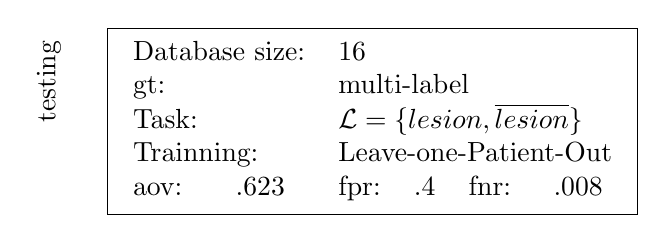
\begin{tikzpicture}[remember picture]
  \tikzstyle{noMargin} = [inner sep=0mm, outer sep=0mm]
  %\node[draw, noMargin, remember picture, anchor=north west,
  %minimum width = 3cm,
  %label={[label distance=-0.8cm,text depth=15pt,rotate=90]left:description}
  %](methodTech){
  %  \qquad
  %  \begin{tabular}{lll}
  %    \multicolumn{3}{l}{technology used for:}\\ 
  %    \multicolumn{2}{l}{\qquad detection}& \myCoord{mlInit}\\
  %    \multicolumn{2}{l}{\qquad segmentation}\\
  %    \multicolumn{2}{l}{\qquad post-processing}&\myCoord{mlFin}\\
  %    $\mathcal{S}$: & \multicolumn{2}{l}{Quick-Shift super-pixels}\\
  %    $\arg \min (U(\cdot))$:&\multicolumn{2}{l}{\acl{gc}}\\
  %    $D(\cdot)$:&\multicolumn{2}{l}{\tikz[noMargin, baseline=(img.north)]{\node[noMargin](img){\includegraphics[width=1cm]{vcues}};}}\\
  %    &\multicolumn{2}{l}{\acs{rbf}-\acs{svm}}\\
  %    $V(\cdot,\cdot)$:&\multicolumn{2}{l}{Homogenity}\\
  %  \end{tabular}
  %};
  %\node[yshift=2pt,remember picture, overlay, nodeBase, mlStyle, fit= (mlInit) (mlFin)]{};
\node[draw, %below= 2pt of methodTech,
minimum width = 3.9cm,
  label={[label distance=-0.5cm,text depth=15pt,anchor=south, rotate=90]left:testing}
  ](testingNode){
    \begin{tabular}{lclclc}
      \multicolumn{2}{l}{Database size:} & \multicolumn{4}{l}{$16$} \\
      \multicolumn{2}{l}{\ac{gt}:}       & \multicolumn{4}{l}{multi-label} \\
      \multicolumn{2}{l}{Task:}          & \multicolumn{4}{l}{$\mathcal{L} = \{\text{lesion}, \overline{\text{lesion}}\}$} \\
      \multicolumn{2}{l}{Trainning:}     & \multicolumn{4}{l}{Leave-one-Patient-Out}\\
      \ac{aov}:      & .623                                                                               & \acs{fpr}: & .4 & \acs{fnr}: & .008
    \end{tabular}
    };
%  \node[
%        draw=red,
%        minimum width=\textwidth,
%        fit=(current bounding box.north west) (current bounding box.south east),
%      ]at (current bounding box.center){};
\end{tikzpicture}

};
\end{tikzpicture}
 }
    %\caption{{\small comparison}}
    \label{fig:surveyResults:comparison}
  \end{subfigure}
  \caption{Quantitative results compilation and comparison}
  \label{fig:surveyResults}
\end{figure}

A 16 \ac{bus} images dataset with accompanying multi-label \ac{gt} delineating all the structures present in the images has been used to evaluate the proposed methodology for lesion segmentation application.
Every image in the dataset presents a single lesion with a variable extension. 
The size of the lesions ranges from under $1/100$ to over $1/5$ of the image size.
The dataset is composed of cysts, \acp{fa}, \acp{dic} and \acp{ilc}. This dataset is now publicly available at \texttt{http://*************}

Due to the lack of publicly available dataset and source code, a comparison between the
different methods is limited to a compilation of results provided
by the different authors and express them with common metric, as reported in~\cite{massich2013phd}.
This information has been replicated in Fig.\,\ref{fig:surveyResults} using the \ac{aov} metric.

Figure~\ref{fig:surveyResults} is divided in three main parts: (i) a table on the top summarizes the core stages of each study framework, (ii) a legend box on the right side informing of our testing setup and (iii) a comparison of the different metrics in a radial manner. An extra element is also represented in this radial representation: a blue swatch delimited by two blue dashed lines. The boundaries of this swatch correspond to the performance of some expert radiologists based on an inter- and intra-observer experiments carried out by Pons et al.~\cite{gerard2013}.
It is interesting to note that some methodologies outperform this swatch.
A publicly available dataset should allow a better comparison in that regard.

The results point out the inherent capabilities of \ac{ml} to cope with data scalability and variability, induce its usage in conjunction with larger datasets.
Whereas, \ac{acm} methodologies show its effectiveness for model the boundary in a natural manner.
% The ability of \ac{ml} to cope with data variability, as well as its need of data, explains why these methodologies
% have been tested, whereas the ability of \ac{acm} methods in constraining the boundary lead to slightly better results in terms of \ac{aov}.

For our proposed framework, the performance in terms of \ac{aov} lies within the state-of-the-art despite its final delineation 
limited by the capacity of the super-pixels to snap the desired boundary.
Figure~\ref{fig:results} shows some qualitative results where the limitations of labeling super-pixels when compared to hand-drawn \ac{gt}.
Figure~\ref{fig:results} also illustrates the influence of the pair-wise term.
%depicts the differences between the delineation resulting from a proper labeling of the super-pixels and the one from the \ac{gt}.

%The iconography used for the table, relates methodology stages, the technology used and if the stages have been treated separately or as a single processing.
%The figure, also arranges the information in a radial manner for direct visual comparison.



%Comparing these results, the inconvenience of unexciting public data can be obviously highlighted, since that several of these results outperform the manual delineations performed in Pons et al.~\cite{gerard2013} on the dataset here used.


% Figure~\ref{fig:results} shows qualitative results, whereas the quantitative results from the best configuration are reported as a table in Fig.\,\ref{fig:surveyResults}. %~\cite{massich2013phd}.

%Despite the fact that a \ac{fpr} of $0.4$ seems significant, based on our experiments most of the images produce no \ac{fp} lesions.
%However, images with \ac{fp} lesions, are likely to produce more several of them as shown in \cref{fig:results}c-e.
%The amount of \ac{fp} lesions can be trimmed by applying a higher cost in the pairwise therm (compare \cref{fig:resuts:smallPWterm} and \cref{fig:results:bigPWterm}.
%Nevertheless, a severe increasing of the pairwise cost also increases the \ac{fnr} since some lesions are missed due to over-smoothing. %~\cite{massich2013phd}.
%The situation of having a larger \ac{fnr} is less desirable than reducing the \ac{fpr}. 
%The \ac{fnr} reported in \cref{fig:surveyResults:method} is caused by an image within the dataset that its lesion is fully contained in a single super-pixel and still around $20\%$ of this super-pixel's area is healty tissue. 

% Due to the lack of publicly available data and source code, there is no manner to perform a comparison further apart of compiling the results reported in the literature.
% Based on \emph{******** et al.} the state-of-the-art methodologies found in the literature, the results are summarized in Fig.\,\ref{fig:surveyResults} and are reported in terms of \ac{aov} for comparison purposes. The references equivalence can be found in~\cite{massich2013phd}
%compiles relevant metholodologies relevant methodologies found in the literature 
%The table in \Cref{fig:surveyResults:survey} complies the evaluation reported by the authors of the most relevant methodologies found in the literature. %~\cite{massich2013phd}.
%Details about the methodologies proposed in the literature can also be found in the aforesaid table.
%Specifically it is detailed the category of technique been used for detecting the lesions, segmenting it and post-process the delineations (if any).
%The studied categories are: \ac{ml}, \ac{acm} and others.
%if the those stages are treated as independent and connected in a daisy-chain fashion, or otherwise the stages are addressed in an atomic manner.


%\Cref{fig:surveyResults:comparison} renders the information present in \cref{fig:surveyResults:survey} and \cref{fig:surveyResults:method} in a visual manner compare all the results at once.
%The methodologies arranged in a radial fashion and grouped by its most representative technology category. 
%In red it can be found a small, medium and large categorization of the dataset reported for testing.
%The concentric circles represent \ac{aov}. 
%The blue line correspond to the \ac{aov} results reported in the literature, whereas the black line indicates the \ac{aov} our framework scored in our testing.

%\footnote{The dataset used for testing the framework here proposed corresponds to the subset of images used by Pons et al.~\cite{gerard2013} that have accompanying multi-labelled \ac{gt}.}.

%%% Local Variables: 
%%% mode: latex
%%% TeX-master: "../../master.tex"
